\chapter{Lunar-Solar Syzygies and Eclipses}
% !TEX root = ../Almagest.tex

\section{Syzygies}
Let $\lambda_S$ and $\lambda_M$ represent the ecliptic longitudes
of the Sun and the Moon, respectively. The lunar-solar {\em elongation}\/  is defined
\begin{equation}
D = \lambda_M - \lambda_S.
\end{equation}
Because the  Moon is only visible because of light reflected from the Sun, there is a fairly obvious relationship between lunar-solar elongation and lunar
phase. See Figure~\ref{fphase}. For instance, a {\em new moon}\/ corresponds to 
$D = 0^\circ$, a {\em quarter moon}\/ to $D = 90^\circ$ or $270^\circ$, and a {\em full moon}\/ to $D = 180^\circ$. New moons and full moons are collectively known as lunar-solar {\em syzygies}. (From the Greek
συζυγία, meaning ``yoking together'' or conjuction.)

\begin{figure}[h]
\centerline{\includegraphics[height=3in]{epsfiles/phase.eps}}
\caption{The phases of the Moon.}\label{fphase}
\end{figure}

\section{Lunar-Solar Elongation Model}
We can determine the  lunar-solar elongation  by combining the solar and
lunar models described in the previous two chapters. Our elongation model is as
follows:
\begin{align}
\bar{D} &= \bar{\lambda}_M - \bar{\lambda}_S,\\[0.5ex]
q_1 &= 2\,e_M\,\sin M_M + 1.430\,e^2\,\sin 2M_M,\\[0.5ex]
q_2 &= 0.422\,e_M\,\sin (2\bar{D} - M_M),\\[0.5ex]
q_3 &= 0.211\,e_M\,(\sin 2\bar{D} - 0.066\,\sin \bar{D}),\\[0.5ex]
q_4 &= -(0.051\,e_M+2\,e_S)\,\sin M_S - (5/4)\,e_S^{\,2}\,\sin 2 M_S,\\[0.5ex]
q_5&= -0.038\,e_M\,\sin 2 \bar{F}_M,\\[0.5ex]
D &= \bar{D} + q_1+q_2+q_3+q_4+q_5.
\end{align}
Here, $e_S$, $M_S$,  and $\bar{\lambda}_S$  are the eccentricity, mean anomaly,  and mean longitude  of the Sun's apparent orbit about the Earth, respectively. Moreover, $e_M$,
$M_M$, $\bar{\lambda}_M$, and $\bar{F}_M$ are the eccentricity, 
mean anomaly, mean longitude, and mean argument of latitude of
the Moon's orbit, respectively.

The lunar-solar elongation can be calculated with the aid of Tables~\ref{telon} and \ref{telona}.
Table~\ref{telon} allows the mean lunar-solar elongation, $\bar{D}$, the mean lunar
argument of latitude, $\bar{F}_M$, the mean anomaly of the Sun, $M_S$,
and the mean anomaly of the Moon, $M_M$, to be determined as functions of time.
Table~\ref{telona} specifies the anomalies $q_1$--$q_5$ as functions of their
various arguments.

Tables~\ref{telon} and \ref{telona} contain equivalent information to that contained in the ``Table of conjunctions" (Συνόδων κανόνιον) and the ``Table of full moons" (Πανσελήνων κανόνιον)
that appear in Section~3 of Book~VI of the Almagest.

\section{Determination of Lunar-Solar Elongation}\label{sxxc}
The procedure for using Tables~\ref{telon} and \ref{telona}  to determine the lunar-solar elongation is as follows:
\begin{enumerate}

 \item Determine the fractional Julian day number, $t$, corresponding to the date and time
at which the lunar-solar elongation is to be calculated with the aid of Tables~\ref{kt1}--\ref{kt3}. Form $\Delta t = t-t_0$, where $t_0=2\,451\,545.0$ is the epoch. 

\item Enter Table~\ref{telon} with the digit for each power of 10
in ${\Delta} t$ and take out the corresponding values of $\Delta \bar{D}$, $\Delta \bar{F}_M$,
 $\Delta M_S$, and $\Delta M_M$. If $\Delta t$ is negative then the 
values are minus those shown in the table.
The value of the mean lunar-solar elongation, $\bar{D}$, is the
sum of all the $\Delta\bar{D}$ values plus the value of $\bar{D}$ at the epoch.
Likewise, the value of the mean lunar argument of latitude, $\bar{F}_M$, is the
sum of all the $\Delta\bar{F}_M$ values plus the value of $\bar{F}_M$ at the epoch. Moreover, the value of the solar mean  anomaly, $M_S$, is
the sum of all the $\Delta M_S$ values plus the value of $M_S$ at the epoch. Finally, the value
of the lunar mean anomaly, $M_M$, is the
sum of all the $\Delta M_M$ values plus the value of $M_M$ at the epoch. 
Add as many multiples of $360^\circ$ to $\bar{D}$, $\bar{F}_M$, $M_S$, and $M_M$
as is required to make them all fall in the range $0^\circ$ to $360^\circ$. 

\item Form the five arguments $a_1=M_M$, $a_2=2\bar{D} - M_M$, $a_3=\bar{D}$, $a_4 = M_S$, $a_5=2\bar{F}_M$. Add as
many multiples of $360^\circ$ to the arguments as is required to make them all fall in the range
$0^\circ$ to $360^\circ$. Round each argument to the nearest degree.

\item Enter Table~\ref{telona} with the value of each of the five arguments $a_1$--$a_5$ and take out the
value of each of the five corresponding anomalies $q_1$--$q_5$. It is necessary to interpolate if the arguments are odd.

\item The lunar-solar elongation is given by $D=\bar{D} + q_1+q_2+q_3+q_4+q_5$.
If necessary, convert $D$ into an angle in the range $0^\circ$ to $360^\circ$. 
The decimal fraction can be converted into arc minutes
using Table~\ref{lt6a}. 
\end{enumerate}

In order to facilitate the calculation of syzygies, the previous model has been used to contruct Table~\ref{tnewmoon}, which lists
the dates and fractional Julian day numbers of the first new moons of the years 1900--2099 CE. Two examples
of syzygy calculations are given in the following section.

\section{Example Syzygy Calculations}
\noindent {\em Example 1}: Sixth new moon in 2004 AD:\\
~\\
From Table~\ref{tnewmoon}, the date of first new moon in 2004 AD is 2453026.4 JD. Now, the
lunar-solar elongation increases at the mean rate $n_M - n_S = 13.17639646-0.98564735=12.1907491^\circ$ per day, or
$360^\circ$ in $29.53$ days; the latter  time period is known as a synodic month. Hence, a rough estimate for the
date of the sixth new moon in 2004 AD is five synodic months after that of the first: that is, $2453026.4
+ 5\times 29.53\simeq 2453174.1$ JD. It follows that $\Delta t = 2453174.1-2451545.0=1629.1$ JD. Let us calculate the lunar-solar elongation at this date.
From Table~\ref{telon}:\\
\begin{tabular}{rrrrr}
&&&&\\
$t$(JD) & $ \bar{D}(^\circ)$ & $\bar{F}_M(^\circ)$ & $M_S(^\circ)$ & $M_M(^\circ)$\\[-2ex]
&&&&\\
$+1\,000$ & $310.749$ & $269.350$ & $265.600$ & $104.993$\\
$+600$ & $114.449$ & $17.610$ & $231.360$ & $278.996$\\
$+20$ & $243.815$ & $264.587$ & $19.712$ & $261.300$\\
$+9$ & $109.717$ & $119.064$ & $8.870$ & $117.585$\\
$+.1$ & $1.219$ & $1.323$ & $0.099$ & $1.306$\\
Epoch & $297.864$ & $93.284$ & $357.588$ & $134.916$\\\cline{2-5}
&$1077.813$ & $765.218$ & $883.229$ & $899.096$\\\cline{2-5}
Modulus & $357.813$ & $45.218$ &$163.229$ & $179.096$\\ 
&&&\\
\end{tabular}\\
Thus,
$$
a_1=M_M\simeq 179^\circ,~~~a_2=2\bar{D}-M_M = 2\times 357.813-179.082\simeq 177^\circ,
$$ 
$$
a_3=\bar{D}\simeq 358^\circ,~~~a_4 = M_S\simeq 163^\circ,
$$ 
$$
a_5=2\bar{F}_M = 2\times 45.218\simeq 90^\circ.
$$
Table~\ref{telona} yields $$
q_1(a_1)=0.101^\circ,~~q_2(a_2)= 0.070^\circ,~~q_3(a_3) = -0.045^\circ,
$$
$$q_4(a_4)=-0.596^\circ,~~q_5(a_5)= -0.119^\circ.
$$
 Hence,
$$
D = \bar{D} + q_1+q_2+q_3+q_4+q_5=357.813+0.101+0.070-0.045-0.596-0.119\simeq
357.22^\circ.
$$
Now, the actual new moon takes place when $D=360.00^\circ$. Thus, a far better estimate for the date 
of the sixth new moon in 2004 AD is $2453174.10 +(360.00-357.22)/12.1907491= 2453174.33$ JD.
This corresponds to 20:00 UT on June 17th.

~\\
\noindent {\em Example 2}: Third full moon in 1982 AD\\
~\\
From Table~\ref{tnewmoon}, the fractional Julian day number of first new moon in 1982 AD is 2444994.7 JD, which
corresponds to January 25th. Because there is more than half a synodic month between this event and the
start of year, we conclude that the first full moon in 1982 AD took place before January 25th.  Hence, a rough estimate for the
date of the third full moon in 1982 AD is one and a half synodic months after that of the first new moon; that is, $2444994.7
+ 1.5\times 29.53\simeq 2445039.0$ JD. It follows that $\Delta t = 2445039.0 -2451545.0=-6506.0$ JD. Let us calculate the lunar-solar elongation at
this date.
From Table~\ref{telon}:\\
\begin{tabular}{rrrrr}
&&&&\\
$t$(JD) & $ \bar{D}(^\circ)$ & $\bar{F}_M(^\circ)$ & $M_S(^\circ)$ & $M_M(^\circ)$\\[-2ex]
&&&&\\
$-6\,000$ & $-64.495$ & $-176.102$ & $-153.601$ & $-269.958$\\
$-500$ & $-335.375$ & $-134.675$ & $-132.800$ & $-52.496$\\
$-6$ & $-73.144$ & $-79.376$ & $-5.914$ & $-78.390$\\
Epoch & $297.864$ & $93.284$ & $357.588$ & $134.916$\\\cline{2-5}
&$-175.150$ & $-296.869$ & $65.273$ & $-265.928$\\\cline{2-5}
Modulus & $184.131$ & $63.062$ &$65.273$ & $94.072$\\ 
&&&\\
\end{tabular}\\
Thus,
$$
a_1=M_M\simeq 94^\circ,~~~a_2=2\bar{D}-M_M = 2\times 184.850-94.072\simeq 276^\circ,
$$ 
$$
a_3=\bar{D}\simeq 185^\circ,~~~a_4 = M_S\simeq 65^\circ,
$$ 
$$
a_5=2\bar{F}_M = 2\times 63.062\simeq 126^\circ.
$$
Table~\ref{telona} yields $$
q_1(a_1)=6.239^\circ,~~q_2(a_2)= -1.320^\circ,~~q_3(a_3) = 0.119^\circ,
$$
$$q_4(a_4)=-1.896^\circ,~~q_5(a_5)= -0.097^\circ.
$$
 Hence,
$$
D = \bar{D} + q_1+q_2+q_3+q_4+q_5=184.850+6.239-1.320+0.119-1.896-0.097\simeq
187.895^\circ.
$$
Now, the actual full moon  takes place when $D=180.00^\circ$. Thus, a far better estimate for the date 
of the third full moon in 1982 AD is $2445039.0 +(180.00-187.90)/12.1907491= 2445038.35$ JD.
This corresponds to 20:00  UT on March 9th.

\section{Solar and Lunar Eclipses}
A {\em solar eclipse}---or, more accurately, a lunar-solar occultation---occurs
when the Moon blocks the light of the Sun. Clearly, this is
only possible at a new moon. See Figure~\ref{fphase}. On the other hand,
a {\em lunar eclipse}\/ occurs when the Moon falls into the
shadow of the Earth. Of course, this is only possible at a full moon. It follows that eclipses
can only take place at  lunar-solar syzygies.

In order to determine whether a particular lunar-solar syzygy coincides with an eclipse, we first need to calculate the angular radii of the
Sun, the Moon, and the Earth's shadow in the sky. Using the small angle approximation, the
angular radius of the  Sun is given by $\rho_S = R_S/r_S$, where
$R_S$ is the solar radius, and $r_S$ the Earth-Sun distance. However,
$r_S\simeq a_S\,(1-e_S\,\cos M_S)$, where $a_S$, $e_S$, and $M_S$
are the major radius, eccentricity, and mean anomaly of the Sun's apparent
orbit around the Earth, respectively. (See Chapter~\ref{ckep}.) Hence,
\begin{equation}
\rho_S \simeq \rho_{S\,0}\,(1+e_S\,\cos M_S),
\end{equation}
where $\rho_{S\,0}=R_S/a_S=6.960\times10^5\,{\rm km}/1.496\times 10^8\,{\rm km}\simeq 15.99'$.
Likewise, the angular radius of the Moon is
\begin{equation}
\rho_M\simeq  \rho_{M\,0}\,(1+e_M\,\cos M_M),
\end{equation}
where $\rho_{M\,0} = R_M/a_M =1743\,{\rm km}/384\,399\,{\rm km}\simeq 15.59'$. Here,
$R_M$, $a_M$, $e_M$, and $M_M$ are the radius of the Moon, and the major radius, eccentricity, and mean anomaly of the Moon's orbit, respectively.
As was shown in the previous chapter, lunar parallax causes the
angular position of the Moon in the sky to shift by up to
\begin{equation}
\delta_M = \frac{R_E}{r_M}= \delta_{M\,0}\,(1+e_M\,\cos M_M),
\end{equation}
where $\delta_{M\,0} = R_E/a_M = 6371\,{\rm km}/384\,399\,{\rm km}=56.98'$. Here, $R_E$ is the
radius of the Earth. Finally, simple trigonometry reveals that
the angular size of the Earth's shadow (that is, umbra) at the radius of the Moon's orbit is
\begin{equation}
\rho_U = \delta_M-\rho_S.
\end{equation}
This can be seen from Figure~\ref{fumbra}.
The radius of the umbra at the position of the Moon is $R_U = R_E-x=
R_E - r_M\,\rho_S$. Hence, the angular radius of the umbra is
$\rho_U = R_U/r_M = \delta_M-\rho_S$. Incidentally,
the identification of two of the angles in the figure with $\rho_S=R_S/r_S$ follows
because $R_S\gg R_E$.

\begin{figure}
\centerline{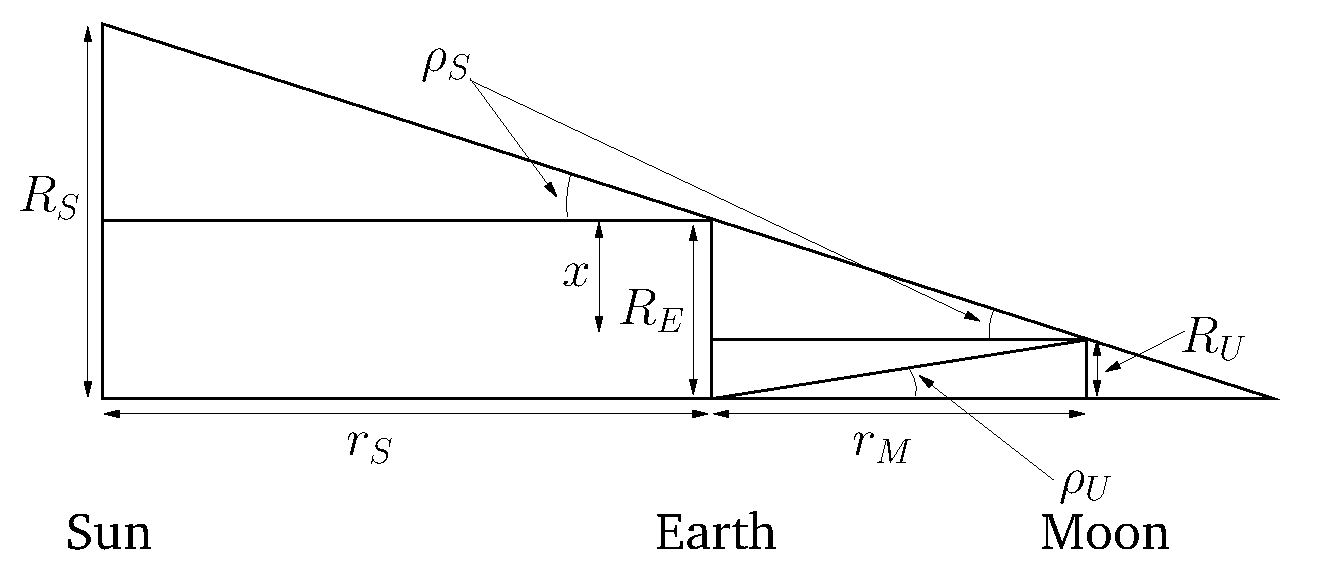
\includegraphics[height=2.5in]{epsfiles/umbra.eps}}
\caption{The Earth's umbra.}\label{fumbra}
\end{figure}

A solar eclipse does not take place every new moon,
nor a lunar eclipse every full moon, because of the inclination of the
Moon's orbit to the ecliptic plane, which causes the Moon to
pass either above or below the Sun, or the Earth's shadow, respectively, in the majority of cases. It follows
that the critical parameter that determines the occurrence of eclipses is
the ecliptic latitude of the Moon at syzygy, $\beta_{syz}$. Of course, once
the date  and time of a syzygy has been established, $\beta_{syz}$
can be calculated from Table~\ref{tmoonb}. However, the lunar argument of latitude, $F$, must first be determined using
\begin{equation}\label{moonla}
F = \bar{F}_M + q_1+q_2+q_3+q_{4'}+q_5,
\end{equation}
where $\bar{F}_M$ comes from Table~\ref{telon}, $q_1$, $q_2$, $q_3$, and $q_5$ are obtained from Table~\ref{telona},
and $q_{4'}$ is the $q_4$ from Table~\ref{tmoona}. For instance, we
have seen that for the third new moon of 1982 AD, $\bar{F}_M=63.131$, $M_S\simeq 65^\circ$, $q_1=6.239^\circ$, $q_2=-1.320^\circ$, $q_3=0.119^\circ$, and $q_5=-0.097^\circ$. According to Table~\ref{tmoona}, $q_{4'}(M_S) = -0.145^\circ$. Hence, $F =  \bar{F}_M + q_1+q_2+q_3+q_{4'}+q_5
=63.139+6.239-1.320+0.119-0.145-0.097=67.926\simeq 68^\circ$. 
It follows from Table~\ref{tmoonb} that $\beta_{syz} = 4.790^\circ\simeq 4^\circ 47'$. 

\begin{figure}
\centerline{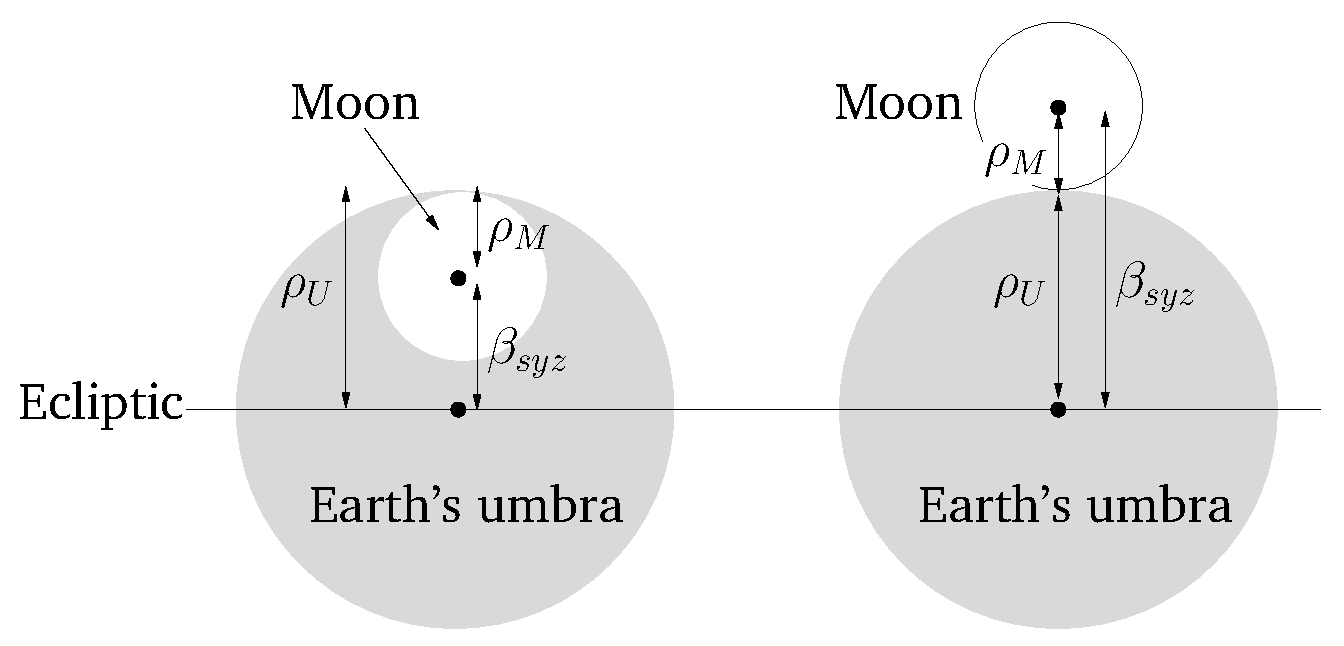
\includegraphics[height=2.5in]{epsfiles/totalm.eps}}
\caption{The limiting cases for a total lunar eclipse (left) and a partial lunar eclipse (right).}\label{fmoonec}
\end{figure}

The criterion for
a lunar eclipse is particularly simple, because it is not
complicated by lunar parallax. A {\em total lunar eclipse}, in which the Moon is
completely immersed in the Earth's shadow, must take place at a
full moon if $|\beta_{syz}| < \rho_U-\rho_M$ (see Figure~\ref{fmoonec}),
or equivalently
\begin{equation}
|\beta_{syz}| < \delta_M-\rho_M-\rho_S,
\end{equation}
and either a total or a {\em partial lunar eclipse}, in which the Moon is only
partially immersed in the Earth's shadow, must take place if
$ |\beta_{syz}| < \rho_U+\rho_M$ (see Figure~\ref{fmoonec}),
or  equivalently
\begin{equation}
|\beta_{syz}| < \delta_M+\rho_M-\rho_S.
\end{equation}
 Note that lunar eclipses are simultaneously
visible at all observation sites on the Earth for which the Moon is
above the horizon, because the Earth's shadow is larger than the Moon, and the relative position of the Moon and the Earth's shadow is not affected by parallax
(because both the Moon and the shadow are the same distance from the Earth).

 The criterion for a solar eclipse is modified by lunar parallax, which causes the angular position of the Moon relative to the Sun to shift by up to $\delta_M$ from its geocentric position. The amount of the shift
 depends on the observation site. However, a site can always be found
 at which the shift takes its maximum value in any particular direction.
 Note that the Sun has negligible parallax, because it is much further away from the Earth than the Moon. Taking parallactic shifts into account, a {\em total solar eclipse}, in which the Sun is totally obscured by the Moon,
must take place if $\rho_M>\rho_S$ and
 \begin{equation}
 |\beta_{syz}| < \delta_M + \rho_M - \rho_S,
 \end{equation}
 an {\em annular solar eclipse}, in which all of the Sun apart from
 a thin outer ring is obscured by the Moon, must take place if
 $\rho_S>\rho_M$ and
 \begin{equation}
 |\beta_{syz}| < \delta_M +  \rho_S-\rho_M,
 \end{equation}
 and either a total, an annular,  or a {\em partial solar eclipse}, in which the
 Sun is only partially obscured by the Moon,  must take place if
 \begin{equation}
    |\beta_{syz}|< \delta_M + \rho_M + \rho_S.
  \end{equation}
As a consequence of lunar parallax, and the fact that the angular sizes of the Sun and Moon in the sky are very similar, solar eclipses are only visible in very localized regions of the Earth. Note, finally, that the previous criteria represent
necessary, but not sufficient, conditions for the occurrence of the various eclipses with which
they are associated. This is the case because the point of closest
approach of the Moon and the Earth's shadow, in the case of a
lunar eclipse, and the Moon and Sun, in the case of a solar eclipse, does
not necessarily occur exactly at the syzygy, due to the inclination
of the Moon's orbit to the ecliptic. However, because the said inclination
is fairly gentle, the previous criteria turn out to be very accurate
predictors of eclipses. 

The criterion for a total lunar eclipse can be written $|\beta_{syz}|< \beta_{Mt}$, where
\begin{equation}\label{elt}
\beta_{Mt} = 25.41' + \delta\beta_1(M_M)-\delta\beta_2 (M_M)-\delta\beta_3(M_S).%\label{ae137}
\end{equation}
Here, the functions $\delta\beta_1=\delta_{M\,0}\,e_M\,\cos M_M$, $\delta\beta_2= \rho_{M\,0}\,e_M\,\cos M_M$, and $\delta\beta_3=\rho_{S\,0}\,e_S\,\cos M_S$
are tabulated in Table~\ref{tsyzb}. The criterion for any type of
lunar eclipse becomes $|\beta_{syz}|< \beta_{M}$, where
\begin{equation}\label{elp}
\beta_{M} = 56.59' +  \delta\beta_1(M_M)+\delta\beta_2 (M_M)-\delta\beta_3(M_S).
\end{equation}
The criterion for a total  solar eclipse can
be written $|\beta_{syz}|<\beta_{St}$ and $\beta_{St}>\beta_{Sa}$, where
\begin{equation}\label{est}
\beta_{St} = 56.59' +  \delta\beta_1(M_M)+\delta\beta_2 (M_M)-\delta\beta_3(M_S),
\end{equation}
and
\begin{equation}\label{esa}
\beta_{Sa} = 57.39' +  \delta\beta_1(M_M)-\delta\beta_2 (M_M)+\delta\beta_3(M_S),
\end{equation}
The criterion for an annular  solar eclipse is $|\beta_{syz}|<\beta_{Sa}$ and $\beta_{Sa}>\beta_{St}$.
Finally, 
the criterion for any
type of solar eclipse is $|\beta_{syz}|< \beta_{S}$, where
\begin{equation}\label{esp}
\beta_{S} = 88.57' +  \delta\beta_1(M_M)+\delta\beta_2 (M_M)+\delta\beta_3(M_S).%\label{ae140}
\end{equation}

\section{Example Eclipse Calculations}
Let us use our model to examine the lunar-solar syzygies of the year
1992 AD in order to see whether any of them were associated with solar or
lunar eclipses. The following  table  shows the dates and times of the new moons
of 1992 AD, calculated using the method described in Section~\ref{sxxc}. Also shown is the magnitude of the Moon's ecliptic latitude
at each syzygy, $|\beta_{syz}|$, calculated from 
Eqaution~(\ref{moonla}) and Table~\ref{tmoonb}, as well as the critical values of
this parameter for a general,  total, and annular solar eclipse. The latter are calculated from
Equations~(\ref{est})--(\ref{esp}) with the aid of Table~\ref{tsyzb}. It can be seen that
the criterion for a total solar eclipse (that is, $|\beta_{syz}|< \beta_{St}$ and $\beta_{St}>\beta_{Sa}$) is satisfied for the syzygy marked with a T,  the criterion for an annular solar eclipse (that is, $|\beta_{syz}|< \beta_{Sa}$ and $\beta_{Sa}>\beta_{St}$) for the syzygy marked with an A,
and
the criterion for a partial solar eclipse  (that is, $\beta_{St},\beta_{Sa}<|\beta_{syz}|< \beta_{S}$)  for the syzygy marked with a P. It is easily verified
that a total solar eclipse, an annular solar eclipse, and a partial solar eclipse did indeed
take place in 1992 AD at the dates and times indicated.\\
\begin{tabular}{cccccrc}
&&&&&&\\
Date & Time (UT) & $\beta_{S}(')$ & $\beta_{St}(')$ & $\beta_{Sa}(')$ & $|\beta_{syz}|(')$\\\hline
04/01/1992  &23:00   &85.0   &52.5   &55.5   &22.8  &A\\
03/02/1992  &16:00   &84.9   &52.5   &55.4  &177.9  & \\
04/03/1992  &09:00   &85.7   &53.4   &55.8  &282.7  & \\
03/04/1992  &00:00   &87.1   &55.1   &56.5  &307.5  & \\
02/05/1992  &14:00   &88.7   &57.0   &57.4  &245.8  & \\
01/06/1992  &01:00   &90.3   &58.8   &58.3  &115.6  & \\
30/06/1992  &12:00   &91.5   &60.1   &59.0   &46.3  &T\\
29/07/1992  &21:00   &92.2   &60.7   &59.4  &195.3  & \\
28/08/1992  &05:00   &92.3   &60.7   &59.5  &290.2   &\\
26/09/1992  &14:00   &91.8   &59.9   &59.2  &304.8   &\\
26/10/1992  &00:00   &90.7   &58.5   &58.7  &234.8   &\\
24/11/1992  &11:00   &89.2   &56.8   &57.8   &99.3   &\\
24/12/1992  &01:00   &87.4   &54.9   &56.9   &64.3  &P\\
&&&&&&\\
\end{tabular}

The following table shows the dates and times of the full moons
of 1992 AD. Also shown is the magnitude of the Moon's ecliptic latitude
at each syzygy, as well as the critical values of
this parameter for a general and a total lunar eclipse. The latter are calculated from
Equations~(\ref{elp}) and (\ref{elt}), respectively, with the aid of Table~\ref{tsyzb}. It can be seen that
the criterion for a total lunar eclipse (that is, $|\beta_{syz}|< \beta_{Mt}$) is satisfied for the syzygy  marked with a T, whereas
the criterion for a partial lunar eclipse  (that is, $\beta_{Mt}<|\beta_{syz}|< \beta_{M}$) is satisfied for the syzygy marked with a P. It is easily verified
that a total lunar eclipse, and a partial lunar eclipse did indeed
take place in 1992 AD at the dates and times indicated.\\
\begin{tabular}{ccccrc}
&&&&&\\
Date & Time (UT) & $\beta_{M}(')$ & $\beta_{Mt}(')$ & $|\beta_{syz}|(')$\\\hline
19/01/1992  &20:00   &60.3   &27.4  &104.2   &\\
18/02/1992  &05:00   &60.1   &27.3  &237.8   &\\
18/03/1992  &14:00   &59.3   &26.9  &305.6   &\\
17/04/1992  &01:00   &57.9   &26.2  &288.5   &\\
16/05/1992  &13:00   &56.3   &25.3  &190.8   &\\
15/06/1992  &03:00   &54.7   &24.4  & 39.4  &P\\
14/07/1992  &20:00   &53.4   &23.7  &123.4  & \\
13/08/1992  &13:00   &52.8   &23.3  &251.6  & \\
12/09/1992  &05:00   &53.1   &23.5  &308.6  & \\
11/10/1992  &21:00   &54.3   &24.1  &278.2  & \\
10/11/1992  &12:00   &55.8   &24.9  &169.6  & \\
10/12/1992  &01:00   &57.5   &25.8   &13.8  &T\\
08/01/1993  &12:00   &59.0   &26.7  &145.4  & \\
\end{tabular}

\section{Eclipse Statistics}
Consider a very large collection of lunar-solar syzygies. For such a collection,
we expect the lunar argument of latitude, $F$, the lunar mean anomaly, $M_M$,
and the solar mean anomaly, $M_S$, to be statistically independent of one another, and randomly distributed in
the range $0^\circ$ to $360^\circ$. Using this
insight, we can easily calculate the probability that a new moon is coincident with a
solar eclipse, or a full moon with a lunar eclipse, using Equation~(\ref{emoonlat})
and the criteria (\ref{elt})--(\ref{esp}).
For a new moon we find:\\
\begin{tabular}{lr}
&\\
Probability of total solar eclipse: &$4.2\%$\\
Probability of annular solar eclipse: &$7.7\%$\\
Probability of partial solar eclipse: &$6.6\%$\\
Probability of any solar eclipse:&$18.5\%$\\
&\\
\end{tabular}\\
 For a full moon we get:\\
\begin{tabular}{lr}
&\\
Probability of total lunar eclipse:& $5.2\%$\\
Probability of partial lunar eclipse: & $6.5\%$\\
Probability of any lunar eclipse:&$11.7\%$\\
&\\
\end{tabular}\\
Thus, we can see that, over a long  period of time, the ratio of the number of total/annular solar eclipses to the number of partial solar
eclipses is about 9/5, whereas the ratio of the number of partial 
lunar eclipses to the number of total lunar eclipses is approximately 5/4. Furthermore,
the ratio of the number of solar eclipses to the number of lunar eclipses
is about 11/7. Because there are 12.37 synodic months in a year, the
mean number of solar eclipses per year is approximately $12.37\times 0.185\simeq 2.3$,
whereas the mean number of lunar eclipses per year is about $12.37\times 0.117\simeq 1.4$. Clearly, solar eclipses are more  common that lunar
eclipses. On the other hand, at a given observation site on the Earth, lunar eclipses
are much more common than solar eclipses, because the former are visible
 over all regions of the Earth for which the Moon is above the horizon, whereas the latter are only visible in a very localized
region.

\section{Eclipse Cycles}
Now, $223$ synodic months corresponds to $6585.413$ days, which corresponds to $238.99$ anomalistic months and $242.00$ draconic months. 
This implies that if a solar eclipse takes place at a given new moon then, $223$ new moons later, the Moon's perigee and ascending node will be found in almost
the exact same positions, which 
 implies that the Moon's ecliptic latitude, as well as $\beta_{St}$, $\beta_{Sa}$, and $\beta_S$, will take almost exactly the same values. Hence, another solar eclipse is almost
certain to happen $223$ new moons after a given eclipse. The same reasoning leads to the conclusion that if a lunar eclipse takes place at
a given full moon then another eclipse is almost certain to occur 223 full moons later. It can easily be demonstrated that there is no number of
synodic months less than $233$ that corresponds to integer numbers of both anomalistic and draconic months. Hence, the time period
of $223$ synodic months, which is (mistakenly) called the {\em saros}, is the minimum (almost) guaranteed period on which solar and lunar eclipses repeat. 

\clearpage
\begin{table}
\centering
\begin{tabular}{rrrrr|rrrrr}
$\Delta t$(JD)& $\Delta \bar{D}(^\circ)$ &  $\Delta \bar{F}_M(^\circ)$ & $\Delta M_S(^\circ)$& $\Delta M_M (^\circ)$ & $\Delta t$(JD) & $\Delta \bar{D}(^\circ)$ & $\Delta \bar{F}_M(^\circ)$ 
&$\Delta M_S(^\circ)$ & $\Delta M_M(^\circ)$\\ \hline
&&&&&&&&&\\[-1.75ex]
10\,000 & 227.491 & 173.503 & 136.002 & 329.930 & 1\,000 & 310.749 & 269.350 & 265.600 & 104.993\\
20\,000 &  94.982 & 347.005 & 272.005 & 299.859 & 2\,000 & 261.498 & 178.701 & 171.200 & 209.986\\
30\,000 & 322.473 & 160.508 &  48.007 & 269.788 & 3\,000 & 212.247 &  88.051 &  76.801 & 314.979\\
40\,000 & 189.964 & 334.011 & 184.010 & 239.718 & 4\,000 & 162.996 & 357.401 & 342.401 &  59.972\\
50\,000 &  57.455 & 147.513 & 320.012 & 209.648 & 5\,000 & 113.746 & 266.751 & 248.001 & 164.965\\
60\,000 & 284.947 & 321.016 &  96.015 & 179.577 & 6\,000 &  64.495 & 176.102 & 153.601 & 269.958\\
70\,000 & 152.438 & 134.519 & 232.017 & 149.506 & 7\,000 &  15.244 &  85.452 &  59.202 &  14.951\\
80\,000 &  19.929 & 308.022 &   8.020 & 119.436 & 8\,000 & 325.993 & 354.802 & 324.802 & 119.944\\
90\,000 & 247.420 & 121.524 & 144.022 &  89.366 & 9\,000 & 276.742 & 264.152 & 230.402 & 224.937\\
&&&&&&&&&\\
100 & 139.075 & 242.935 &  98.560 & 226.499 & 10 & 121.907 & 132.294 &   9.856 & 130.650\\
200 & 278.150 & 125.870 & 197.120 &  92.999 & 20 & 243.815 & 264.587 &  19.712 & 261.300\\
300 &  57.225 &   8.805 & 295.680 & 319.498 & 30 &   5.722 &  36.881 &  29.568 &  31.950\\
400 & 196.300 & 251.740 &  34.240 & 185.997 & 40 & 127.630 & 169.174 &  39.424 & 162.600\\
500 & 335.375 & 134.675 & 132.800 &  52.496 & 50 & 249.537 & 301.468 &  49.280 & 293.250\\
600 & 114.449 &  17.610 & 231.360 & 278.996 & 60 &  11.445 &  73.761 &  59.136 &  63.900\\
700 & 253.524 & 260.545 & 329.920 & 145.495 & 70 & 133.352 & 206.055 &  68.992 & 194.550\\
800 &  32.599 & 143.480 &  68.480 &  11.994 & 80 & 255.260 & 338.348 &  78.848 & 325.199\\
900 & 171.674 &  26.415 & 167.040 & 238.494 & 90 &  17.167 & 110.642 &  88.704 &  95.849\\
&&&&&&&&&\\
1 &  12.191 &  13.229 &   0.986 &  13.065 & 0.1 &   1.219 &   1.323 &   0.099 &   1.306\\
2 &  24.381 &  26.459 &   1.971 &  26.130 & 0.2 &   2.438 &   2.646 &   0.197 &   2.613\\
3 &  36.572 &  39.688 &   2.957 &  39.195 & 0.3 &   3.657 &   3.969 &   0.296 &   3.919\\
4 &  48.763 &  52.917 &   3.942 &  52.260 & 0.4 &   4.876 &   5.292 &   0.394 &   5.226\\
5 &  60.954 &  66.147 &   4.928 &  65.325 & 0.5 &   6.095 &   6.615 &   0.493 &   6.532\\
6 &  73.144 &  79.376 &   5.914 &  78.390 & 0.6 &   7.314 &   7.938 &   0.591 &   7.839\\
7 &  85.335 &  92.605 &   6.899 &  91.455 & 0.7 &   8.534 &   9.261 &   0.690 &   9.145\\
8 &  97.526 & 105.835 &   7.885 & 104.520 & 0.8 &   9.753 &  10.583 &   0.788 &  10.452\\
9 & 109.717 & 119.064 &   8.870 & 117.585 & 0.9 &  10.972 &  11.906 &   0.887 &  11.758\\
\end{tabular}
\caption{Mean motion of the lunar-solar elongation.  Here, $\Delta t = t-t_0$, $\Delta \bar{D}= \bar{D}-\bar{D}_0$, $\Delta \bar{F}_M= \bar{F}_M-\bar{F}_{M\,0}$,  
$\Delta M_S = M_S - M_{S\,0}$, and $\Delta M_M= M_M-M_{M\,0}$. 
At epoch  ($t_0 = 2\,451\,545.0$ JD), $\bar{D}_0 = 297.864^\circ$, $\bar{F}_{M\,0} = 93.284^\circ$,
$M_{S\,0} = 357.588^\circ$, and $M_{M\,0} = 134.916^\circ$. }\label{telon}
\end{table}

\newpage
\begin{table}\centering
\small{ \begin{tabular}{crrrrr|crrrrr}
Arg. ($^\circ$) & $q_1(^\circ)$  & $q_2(^\circ)$ & $q_3(^\circ)$ & $q_4(^\circ)$  & $q_5(^\circ)$ &
Arg. ($^\circ$) & $q_1(^\circ)$  & $q_2(^\circ)$ & $q_3(^\circ)$ & $q_4(^\circ)$  & $q_5(^\circ)$  \\\hline
&&&&&&&&&&&\\[-1.75ex]
000/(360) &  0.000 &  0.000 &  0.000 & $-$0.000 & $-$0.000 & 090/(270) &  6.289 &  1.327 & $-$0.044 & $-$2.075 & $-$0.119\\
002/(358) &  0.237 &  0.046 &  0.045 & $-$0.074 & $-$0.004 & 092/(268) &  6.268 &  1.326 & $-$0.090 & $-$2.073 & $-$0.119\\
004/(356) &  0.473 &  0.093 &  0.089 & $-$0.148 & $-$0.008 & 094/(266) &  6.239 &  1.324 & $-$0.136 & $-$2.067 & $-$0.119\\
006/(354) &  0.709 &  0.139 &  0.133 & $-$0.221 & $-$0.012 & 096/(264) &  6.203 &  1.320 & $-$0.181 & $-$2.060 & $-$0.119\\
008/(352) &  0.943 &  0.185 &  0.177 & $-$0.294 & $-$0.017 & 098/(262) &  6.160 &  1.314 & $-$0.226 & $-$2.050 & $-$0.118\\
010/(350) &  1.176 &  0.230 &  0.219 & $-$0.367 & $-$0.021 & 100/(260) &  6.109 &  1.307 & $-$0.270 & $-$2.037 & $-$0.118\\
012/(348) &  1.408 &  0.276 &  0.261 & $-$0.440 & $-$0.025 & 102/(258) &  6.051 &  1.298 & $-$0.313 & $-$2.022 & $-$0.117\\
014/(346) &  1.637 &  0.321 &  0.301 & $-$0.511 & $-$0.029 & 104/(256) &  5.986 &  1.288 & $-$0.354 & $-$2.004 & $-$0.116\\
016/(344) &  1.864 &  0.366 &  0.340 & $-$0.583 & $-$0.033 & 106/(254) &  5.915 &  1.276 & $-$0.394 & $-$1.984 & $-$0.115\\
018/(342) &  2.088 &  0.410 &  0.376 & $-$0.653 & $-$0.037 & 108/(252) &  5.836 &  1.262 & $-$0.432 & $-$1.962 & $-$0.114\\
020/(340) &  2.310 &  0.454 &  0.411 & $-$0.723 & $-$0.041 & 110/(250) &  5.751 &  1.247 & $-$0.468 & $-$1.937 & $-$0.112\\
022/(338) &  2.527 &  0.497 &  0.444 & $-$0.791 & $-$0.045 & 112/(248) &  5.660 &  1.230 & $-$0.501 & $-$1.910 & $-$0.111\\
024/(336) &  2.741 &  0.540 &  0.475 & $-$0.859 & $-$0.049 & 114/(246) &  5.562 &  1.212 & $-$0.533 & $-$1.881 & $-$0.109\\
026/(334) &  2.951 &  0.582 &  0.504 & $-$0.926 & $-$0.052 & 116/(244) &  5.458 &  1.193 & $-$0.562 & $-$1.850 & $-$0.107\\
028/(332) &  3.157 &  0.623 &  0.529 & $-$0.991 & $-$0.056 & 118/(242) &  5.348 &  1.172 & $-$0.589 & $-$1.816 & $-$0.106\\
030/(330) &  3.358 &  0.663 &  0.553 & $-$1.055 & $-$0.060 & 120/(240) &  5.233 &  1.149 & $-$0.613 & $-$1.780 & $-$0.103\\
032/(328) &  3.554 &  0.703 &  0.573 & $-$1.118 & $-$0.063 & 122/(238) &  5.111 &  1.125 & $-$0.633 & $-$1.742 & $-$0.101\\
034/(326) &  3.746 &  0.742 &  0.591 & $-$1.179 & $-$0.067 & 124/(236) &  4.985 &  1.100 & $-$0.651 & $-$1.702 & $-$0.099\\
036/(324) &  3.931 &  0.780 &  0.605 & $-$1.239 & $-$0.070 & 126/(234) &  4.853 &  1.074 & $-$0.666 & $-$1.660 & $-$0.097\\
038/(322) &  4.111 &  0.817 &  0.617 & $-$1.297 & $-$0.074 & 128/(232) &  4.716 &  1.046 & $-$0.678 & $-$1.616 & $-$0.094\\
040/(320) &  4.285 &  0.853 &  0.625 & $-$1.354 & $-$0.077 & 130/(230) &  4.575 &  1.017 & $-$0.687 & $-$1.570 & $-$0.092\\
042/(318) &  4.454 &  0.888 &  0.631 & $-$1.409 & $-$0.080 & 132/(228) &  4.428 &  0.986 & $-$0.692 & $-$1.522 & $-$0.089\\
044/(316) &  4.615 &  0.922 &  0.633 & $-$1.462 & $-$0.083 & 134/(226) &  4.277 &  0.955 & $-$0.695 & $-$1.473 & $-$0.086\\
046/(314) &  4.770 &  0.955 &  0.632 & $-$1.513 & $-$0.086 & 136/(224) &  4.122 &  0.922 & $-$0.693 & $-$1.422 & $-$0.083\\
048/(312) &  4.919 &  0.986 &  0.627 & $-$1.562 & $-$0.089 & 138/(222) &  3.963 &  0.888 & $-$0.689 & $-$1.369 & $-$0.080\\
050/(310) &  5.061 &  1.017 &  0.620 & $-$1.609 & $-$0.092 & 140/(220) &  3.799 &  0.853 & $-$0.682 & $-$1.314 & $-$0.077\\
052/(308) &  5.195 &  1.046 &  0.609 & $-$1.655 & $-$0.094 & 142/(218) &  3.632 &  0.817 & $-$0.671 & $-$1.258 & $-$0.074\\
054/(306) &  5.323 &  1.074 &  0.596 & $-$1.698 & $-$0.097 & 144/(216) &  3.462 &  0.780 & $-$0.657 & $-$1.201 & $-$0.070\\
056/(304) &  5.443 &  1.100 &  0.579 & $-$1.739 & $-$0.099 & 146/(214) &  3.288 &  0.742 & $-$0.640 & $-$1.142 & $-$0.067\\
058/(302) &  5.555 &  1.125 &  0.559 & $-$1.778 & $-$0.101 & 148/(212) &  3.111 &  0.703 & $-$0.620 & $-$1.082 & $-$0.063\\
060/(300) &  5.660 &  1.149 &  0.537 & $-$1.815 & $-$0.103 & 150/(210) &  2.931 &  0.663 & $-$0.596 & $-$1.020 & $-$0.060\\
062/(298) &  5.757 &  1.172 &  0.511 & $-$1.849 & $-$0.106 & 152/(208) &  2.748 &  0.623 & $-$0.571 & $-$0.958 & $-$0.056\\
064/(296) &  5.847 &  1.193 &  0.483 & $-$1.881 & $-$0.107 & 154/(206) &  2.562 &  0.582 & $-$0.542 & $-$0.894 & $-$0.052\\
066/(294) &  5.929 &  1.212 &  0.453 & $-$1.911 & $-$0.109 & 156/(204) &  2.375 &  0.540 & $-$0.511 & $-$0.829 & $-$0.049\\
068/(292) &  6.002 &  1.230 &  0.420 & $-$1.938 & $-$0.111 & 158/(202) &  2.184 &  0.497 & $-$0.477 & $-$0.764 & $-$0.045\\
070/(290) &  6.068 &  1.247 &  0.385 & $-$1.963 & $-$0.112 & 160/(200) &  1.992 &  0.454 & $-$0.441 & $-$0.697 & $-$0.041\\
072/(288) &  6.126 &  1.262 &  0.348 & $-$1.985 & $-$0.114 & 162/(198) &  1.798 &  0.410 & $-$0.404 & $-$0.630 & $-$0.037\\
074/(286) &  6.176 &  1.276 &  0.309 & $-$2.006 & $-$0.115 & 164/(196) &  1.603 &  0.366 & $-$0.364 & $-$0.561 & $-$0.033\\
076/(284) &  6.218 &  1.288 &  0.269 & $-$2.023 & $-$0.116 & 166/(194) &  1.406 &  0.321 & $-$0.322 & $-$0.493 & $-$0.029\\
078/(282) &  6.252 &  1.298 &  0.227 & $-$2.038 & $-$0.117 & 168/(192) &  1.207 &  0.276 & $-$0.279 & $-$0.423 & $-$0.025\\
080/(280) &  6.278 &  1.307 &  0.184 & $-$2.051 & $-$0.118 & 170/(190) &  1.008 &  0.230 & $-$0.235 & $-$0.354 & $-$0.021\\
082/(278) &  6.296 &  1.314 &  0.140 & $-$2.061 & $-$0.118 & 172/(188) &  0.807 &  0.185 & $-$0.189 & $-$0.283 & $-$0.017\\
084/(276) &  6.306 &  1.320 &  0.094 & $-$2.068 & $-$0.119 & 174/(186) &  0.606 &  0.139 & $-$0.143 & $-$0.213 & $-$0.012\\
086/(274) &  6.308 &  1.324 &  0.049 & $-$2.073 & $-$0.119 & 176/(184) &  0.404 &  0.093 & $-$0.095 & $-$0.142 & $-$0.008\\
088/(272) &  6.302 &  1.326 &  0.003 & $-$2.075 & $-$0.119 & 178/(182) &  0.202 &  0.046 & $-$0.048 & $-$0.071 & $-$0.004\\
090/(270) &  6.289 &  1.327 & $-$0.044 & $-$2.075 & $-$0.119 & 180/(180) &  0.000 &  0.000 & $-$0.000 & $-$0.000 & $-$0.000\\
\end{tabular}}
\caption{Anomalies of the lunar-solar elongation. The common argument corresponds to
$M_M$, $2\bar{D}-M_M$, $\bar{D}$, $M_S$, and $2\bar{F}_M$ for the case of
$q_1$, $q_2$, $q_3$, $q_4$, and $q_5$, respectively. If the argument is
in parenthesies then the anomalies are minus the values shown
in the table. }\label{telona}
\end{table}

\begin{table}
{\small
\begin{tabular}{cc|cc|cc|cc}
01/1/1900 & 2415021.07 & 18/1/1950 & 2433299.83 & 06/1/2000 & 2451550.25 & 23/1/2050 & 2469829.70\\
20/1/1901 & 2415405.10 & 07/1/1951 & 2433654.33 & 24/1/2001 & 2451934.05 & 12/1/2051 & 2470184.29\\
09/1/1902 & 2415759.37 & 26/1/1952 & 2434038.42 & 13/1/2002 & 2452288.07 & 02/1/2052 & 2470538.61\\
28/1/1903 & 2416143.18 & 15/1/1953 & 2434393.09 & 02/1/2003 & 2452642.34 & 19/1/2053 & 2470922.45\\
17/1/1904 & 2416497.16 & 05/1/1954 & 2434747.59 & 21/1/2004 & 2453026.37 & 08/1/2054 & 2471276.44\\
05/1/1905 & 2416851.26 & 24/1/1955 & 2435131.53 & 10/1/2005 & 2453381.00 & 27/1/2055 & 2471660.25\\
24/1/1906 & 2417235.21 & 13/1/1956 & 2435485.62 & 29/1/2006 & 2453765.09 & 16/1/2056 & 2472014.42\\
14/1/1907 & 2417589.74 & 01/1/1957 & 2435839.60 & 19/1/2007 & 2454119.66 & 05/1/2057 & 2472368.90\\
03/1/1908 & 2417944.40 & 19/1/1958 & 2436223.43 & 08/1/2008 & 2454473.97 & 24/1/2058 & 2472753.00\\
22/1/1909 & 2418328.50 & 09/1/1959 & 2436577.73 & 26/1/2009 & 2454857.81 & 14/1/2059 & 2473107.66\\
11/1/1910 & 2418682.98 & 28/1/1960 & 2436961.75 & 15/1/2010 & 2455211.80 & 03/1/2060 & 2473462.19\\
30/1/1911 & 2419066.89 & 16/1/1961 & 2437316.39 & 04/1/2011 & 2455565.88 & 21/1/2061 & 2473846.12\\
19/1/1912 & 2419420.95 & 06/1/1962 & 2437671.03 & 23/1/2012 & 2455949.82 & 10/1/2062 & 2474200.23\\
07/1/1913 & 2419774.94 & 25/1/1963 & 2438055.06 & 11/1/2013 & 2456304.31 & 29/1/2063 & 2474584.01\\
26/1/1914 & 2420158.78 & 14/1/1964 & 2438409.35 & 01/1/2014 & 2456658.97 & 18/1/2064 & 2474938.03\\
15/1/1915 & 2420513.10 & 02/1/1965 & 2438763.37 & 20/1/2015 & 2457043.05 & 06/1/2065 & 2475292.30\\
05/1/1916 & 2420867.69 & 21/1/1966 & 2439147.16 & 10/1/2016 & 2457397.56 & 25/1/2066 & 2475676.33\\
23/1/1917 & 2421251.81 & 10/1/1967 & 2439501.26 & 27/1/2017 & 2457781.49 & 15/1/2067 & 2476030.96\\
12/1/1918 & 2421606.44 & 29/1/1968 & 2439885.18 & 17/1/2018 & 2458135.58 & 05/1/2068 & 2476385.61\\
02/1/1919 & 2421960.84 & 18/1/1969 & 2440239.70 & 06/1/2019 & 2458489.57 & 23/1/2069 & 2476769.64\\
21/1/1920 & 2422344.71 & 07/1/1970 & 2440594.36 & 24/1/2020 & 2458873.41 & 12/1/2070 & 2477123.96\\
09/1/1921 & 2422698.72 & 26/1/1971 & 2440978.45 & 13/1/2021 & 2459227.70 & 01/1/2071 & 2477478.00\\
28/1/1922 & 2423082.50 & 16/1/1972 & 2441332.94 & 02/1/2022 & 2459582.26 & 20/1/2072 & 2477861.78\\
17/1/1923 & 2423436.61 & 04/1/1973 & 2441687.14 & 21/1/2023 & 2459966.36 & 08/1/2073 & 2478215.85\\
06/1/1924 & 2423791.03 & 23/1/1974 & 2442070.95 & 11/1/2024 & 2460321.00 & 27/1/2074 & 2478599.77\\
24/1/1925 & 2424175.10 & 12/1/1975 & 2442424.94 & 29/1/2025 & 2460705.02 & 16/1/2075 & 2478954.26\\
14/1/1926 & 2424529.77 & 01/1/1976 & 2442779.11 & 18/1/2026 & 2461059.31 & 06/1/2076 & 2479308.92\\
03/1/1927 & 2424884.35 & 19/1/1977 & 2443163.08 & 07/1/2027 & 2461413.34 & 24/1/2077 & 2479693.03\\
22/1/1928 & 2425268.33 & 09/1/1978 & 2443517.66 & 26/1/2028 & 2461797.14 & 14/1/2078 & 2480047.54\\
11/1/1929 & 2425622.50 & 28/1/1979 & 2443901.76 & 14/1/2029 & 2462151.23 & 03/1/2079 & 2480401.77\\
29/1/1930 & 2426006.29 & 17/1/1980 & 2444256.39 & 04/1/2030 & 2462505.61 & 22/1/2080 & 2480785.57\\
18/1/1931 & 2426360.28 & 06/1/1981 & 2444610.80 & 23/1/2031 & 2462889.67 & 10/1/2081 & 2481139.55\\
07/1/1932 & 2426714.48 & 25/1/1982 & 2444994.69 & 12/1/2032 & 2463244.33 & 28/1/2082 & 2481523.38\\
25/1/1933 & 2427098.46 & 14/1/1983 & 2445348.71 & 01/1/2033 & 2463598.93 & 18/1/2083 & 2481877.65\\
15/1/1934 & 2427453.06 & 03/1/1984 & 2445702.73 & 20/1/2034 & 2463982.91 & 07/1/2084 & 2482232.21\\
05/1/1935 & 2427807.72 & 21/1/1985 & 2446086.61 & 09/1/2035 & 2464337.11 & 25/1/2085 & 2482616.33\\
24/1/1936 & 2428191.80 & 10/1/1986 & 2446441.01 & 28/1/2036 & 2464720.92 & 15/1/2086 & 2482970.97\\
12/1/1937 & 2428546.18 & 29/1/1987 & 2446825.06 & 16/1/2037 & 2465074.91 & 04/1/2087 & 2483325.41\\
01/1/1938 & 2428900.28 & 19/1/1988 & 2447179.72 & 05/1/2038 & 2465429.07 & 23/1/2088 & 2483709.30\\
20/1/1939 & 2429284.06 & 07/1/1989 & 2447534.31 & 24/1/2039 & 2465813.06 & 11/1/2089 & 2484063.34\\
09/1/1940 & 2429638.09 & 26/1/1990 & 2447918.30 & 14/1/2040 & 2466167.63 & 30/1/2090 & 2484447.11\\
27/1/1941 & 2430021.96 & 15/1/1991 & 2448272.48 & 02/1/2041 & 2466522.30 & 19/1/2091 & 2484801.19\\
16/1/1942 & 2430376.39 & 04/1/1992 & 2448626.47 & 21/1/2042 & 2466906.36 & 09/1/2092 & 2485155.56\\
06/1/1943 & 2430731.02 & 22/1/1993 & 2449010.28 & 11/1/2043 & 2467260.77 & 27/1/2093 & 2485539.63\\
25/1/1944 & 2431115.14 & 11/1/1994 & 2449364.46 & 30/1/2044 & 2467644.65 & 16/1/2094 & 2485894.29\\
14/1/1945 & 2431469.71 & 01/1/1995 & 2449718.95 & 18/1/2045 & 2467998.68 & 06/1/2095 & 2486248.90\\
03/1/1946 & 2431824.00 & 20/1/1996 & 2450103.02 & 07/1/2046 & 2468352.69 & 25/1/2096 & 2486632.90\\
22/1/1947 & 2432207.84 & 09/1/1997 & 2450457.68 & 26/1/2047 & 2468736.58 & 13/1/2097 & 2486987.11\\
11/1/1948 & 2432561.83 & 28/1/1998 & 2450841.75 & 15/1/2048 & 2469090.97 & 02/1/2098 & 2487341.11\\
29/1/1949 & 2432945.62 & 17/1/1999 & 2451196.14 & 04/1/2049 & 2469445.59 & 21/1/2099 & 2487724.89\\
\end{tabular}}
\caption{Dates and fractional Julian day numbers of the first new moons of the years 1900--2099 AD.}\label{tnewmoon}
\end{table}

\newpage
\begin{table}\centering
\small{ \begin{tabular}{rrrrc}
Arg. ($^\circ$) & $\delta\beta_1(')$ &  $\delta\beta_2(')$ &
 $\delta\beta_3(')$& Arg. ($^\circ$) \\\hline
&&&&\\[-1.75ex]
000/360 &  3.128 &  0.856 &  0.267 & (180)/(180)\\
002/358 &  3.126 &  0.855 &  0.267 & (178)/(182)\\
004/356 &  3.120 &  0.854 &  0.267 & (176)/(184)\\
006/354 &  3.111 &  0.851 &  0.266 & (174)/(186)\\
008/352 &  3.097 &  0.847 &  0.265 & (172)/(188)\\
010/350 &  3.080 &  0.843 &  0.263 & (170)/(190)\\
012/348 &  3.059 &  0.837 &  0.261 & (168)/(192)\\
014/346 &  3.035 &  0.830 &  0.259 & (166)/(194)\\
016/344 &  3.007 &  0.822 &  0.257 & (164)/(196)\\
018/342 &  2.975 &  0.814 &  0.254 & (162)/(198)\\
020/340 &  2.939 &  0.804 &  0.251 & (160)/(200)\\
022/338 &  2.900 &  0.793 &  0.248 & (158)/(202)\\
024/336 &  2.857 &  0.782 &  0.244 & (156)/(204)\\
026/334 &  2.811 &  0.769 &  0.240 & (154)/(206)\\
028/332 &  2.762 &  0.755 &  0.236 & (152)/(208)\\
030/330 &  2.709 &  0.741 &  0.231 & (150)/(210)\\
032/328 &  2.652 &  0.726 &  0.227 & (148)/(212)\\
034/326 &  2.593 &  0.709 &  0.222 & (146)/(214)\\
036/324 &  2.530 &  0.692 &  0.216 & (144)/(216)\\
038/322 &  2.465 &  0.674 &  0.211 & (142)/(218)\\
040/320 &  2.396 &  0.655 &  0.205 & (140)/(220)\\
042/318 &  2.324 &  0.636 &  0.199 & (138)/(222)\\
044/316 &  2.250 &  0.615 &  0.192 & (136)/(224)\\
046/314 &  2.173 &  0.594 &  0.186 & (134)/(226)\\
048/312 &  2.093 &  0.573 &  0.179 & (132)/(228)\\
050/310 &  2.010 &  0.550 &  0.172 & (130)/(230)\\
052/308 &  1.926 &  0.527 &  0.165 & (128)/(232)\\
054/306 &  1.838 &  0.503 &  0.157 & (126)/(234)\\
056/304 &  1.749 &  0.478 &  0.149 & (124)/(236)\\
058/302 &  1.657 &  0.453 &  0.142 & (122)/(238)\\
060/300 &  1.564 &  0.428 &  0.134 & (120)/(240)\\
062/298 &  1.468 &  0.402 &  0.125 & (118)/(242)\\
064/296 &  1.371 &  0.375 &  0.117 & (116)/(244)\\
066/294 &  1.272 &  0.348 &  0.109 & (114)/(246)\\
068/292 &  1.172 &  0.321 &  0.100 & (112)/(248)\\
070/290 &  1.070 &  0.293 &  0.091 & (110)/(250)\\
072/288 &  0.967 &  0.264 &  0.083 & (108)/(252)\\
074/286 &  0.862 &  0.236 &  0.074 & (106)/(254)\\
076/284 &  0.757 &  0.207 &  0.065 & (104)/(256)\\
078/282 &  0.650 &  0.178 &  0.056 & (102)/(258)\\
080/280 &  0.543 &  0.149 &  0.046 & (100)/(260)\\
082/278 &  0.435 &  0.119 &  0.037 & (098)/(262)\\
084/276 &  0.327 &  0.089 &  0.028 & (096)/(264)\\
086/274 &  0.218 &  0.060 &  0.019 & (094)/(266)\\
088/272 &  0.109 &  0.030 &  0.009 & (092)/(268)\\
090/270 &  0.000 &  0.000 &  0.000 & (090)/(270)\\
\end{tabular}}
\caption{Lunar-solar eclipse functions. The  arguments of $\delta\beta_1$, $\delta\beta_2$, and $\delta\beta_3$ are $M_M$, $M_M$, and $M_S$, respectively.  $\delta\beta_1$, $\delta\beta_2$, and  $\delta\beta_3$ take minus the values shown
in the table if their arguments are
in parenthesies. }\label{tsyzb}
\end{table}


